\chapter{FET projects and social media}
This chapter presents an overview of the presence of FET projects on social media. Ut enim ad minim veniam, quis nostrum exercitationem ullam corporis suscipit laboriosam, nisi ut aliquid ex ea commodi consequatur. Quis aute iure reprehenderit in voluptate velit esse cillum dolore eu fugiat nulla pariatur. Excepteur sint obcaecat cupiditat non proident, sunt in culpa qui officia deserunt mollit anim id est laborum.

\section{Data set}
This thesis focuses on the online communication activity of FET projects funded within Horizon 2020. The list of such projects was downloaded on 15th July 2017 from CORDIS, the main portal of the European Commission on results of EU-funded research projects. It consists of 151 projects and it is reported in Appendix \ref{List_of_FET_projects}. For each project, Appendix \ref{List_of_FET_projects} reports information on budget and start and end date, as well as the activated online communication channels. FET projects approved after 15th July 2017 are not considered in this thesis.  

Some of the projects in the list were not considered for this work. Excluded groups were the Flagship and Launchpad projects (see section \ref{The_FET_programme} for a brief description of the two groups), which were not considered representative of FET initiatives in terms of communication effort, as well as projects started after 1st February 2017. 

Flagship projects were disregarded due to their budget.  As the available funding is far superior compared to the other FET projects, the Human Brain Project and the Graphene Flagships can invest larger resources on the communication activity. Thus, the two initiatives are outliers in the considered data set. 

Launchpad projects were not considered for this thesis as their ultimate goal is finding applications of results achieved by other FET projects and have limited interest in communication activity. Moreover, the available budget is relatively small. 

Finally, projects started after 1st February 2017 were disregarded as the time span between this date and the list download was judged insufficient to fully develop and launch an adequate communication activity. The only exception is the DEEP-EST project. In fact, by the time of writing DEEP-EST has already started its online communication activity.    

The lists of the excluded projects are reported in Appendix \ref{Specific_lists_of_FET_projects}. This procedure reduced the number of samples in the data set from 151 to 130.

For some of the analyses in this thesis, the data set of 130 projects was divided into three sub-groups.  The first group consists of the 23 projects active in HPC and the transition to the exascale (see section \ref{FET_and_high-performing_computing}). The second subgroup includes the 12 projects in the field of quantum technologies (see section \ref{FET_and_quantum_technologies}). The third group comprises the other 95 projects. The lists of projects in the HPC and quantume technologies groups are reported in Appendix \ref{Specific_lists_of_FET_projects}. 

\section{Considered channels} \label{Considered_channels}
There exist disparate channels suitable for communication purposes. Those offering the widest audience are provided by the web. Examples are websites and social media. For this reason, FET projects consider the internet as one of the main pillars of their communication strategy.

Different approaches can be considered to assess the use of online communication channels made by FET projects. One quantitative estimate is provided by the fraction of projects active on specific platforms. For this thesis, the following communication channels were considered:   

\begin{description}
 \item [Website] The website is the online channel offering the highest degree of freedom to the owner. It allows the owner to personalise the content, the overall structure and the graphic impact.
 \item [Facebook] Facebook is the most used social media. It offers direct interaction among users and activities are recorded. Nevertheless, it is mainly designed for free time.  
 \item [Twitter] Twitter is very effective for short science-related communication. However, it requires high posting rates and offers less personal interaction compared to Facebook.
 \item [Linkedin] Linkedin is ideal for professional content and enables the creation of closed groups. Nevertheless, interaction among users and outreach within the groups are limited.
 \item [YouTube] YouTube is the world's main platform for video sharing. It provides a very direct communication channel with effective monitoring tools. On the other hand, it does not offer straightforward engagement channels and finding appropriate content may be difficult for users.
 \item [Instagram]Instagram has a very active and rapidly growing community. It requires pictures with strong visual content and offers a limited interaction among users.
 \item [ResearchGate] ResearchGate offers the possibility to share documentation and engage in scientific discussions with researchers. As members are mainly scientists, the community which can be reached is significantly smaller compared to other social networks.  
\end{description}

For each FET projects in appendix \ref{List_of_FET_projects}, a search was performed to find out which online communication platforms among the aformentioned ones had been considered. This search included contacting each project directly. Not for all project was possible to find a contact and in some cases it was not possible to receive an answer (dare numero). For this projects, the author performed a desk search. It cannot be excluded that the desk search did not find all accounts activated by the projects on the aformentioned social channels. It is therefore highly probable that the list of accounts is not complete. Hence, the results presented in this thesis can be considered as inferior limits.   

\section{Overall presence}
Disparate approaches can be considered to assess the use of online communication channels made by FET projects. One quantitative estimate is provided by the fraction of projects which considered the communication channels listed in section \ref{Considered_channels}. 

Out of the ... projects in the data set, ... have created a website, whereas ... have opened accounts on Twitter, ... on Facebook, ... on  Linkedin, ... on YouTube, ... on ResearchGate and ... on Instagram. The results, expressed in percentage, are shown in Figure \ref{Social_media}.

The results show that almost all FET projects have created a website. Facebook and Twitter are the two most popular social media in society and within the FET community. Nevertheless, the fraction of projects which activated a Twitter account is significantly larger than that of facebook. Contrarily to normal people, where facebook is still the most used social media. This is probably due to the fact that Twitter is considered a more suitable tool for scientific communication. YouTube and Instagram are not common communication channels among FET projects. This is probably due to the difficulty of collecting visually impacting material and, in the case of YouTube, the high resources required for the production of high-quality videos. Finally, the number of projects which activated an account on ResearchGate is low. This is probably due to the fact that FET researchers 

\begin{figure}[!t] 
 \begin{center}
 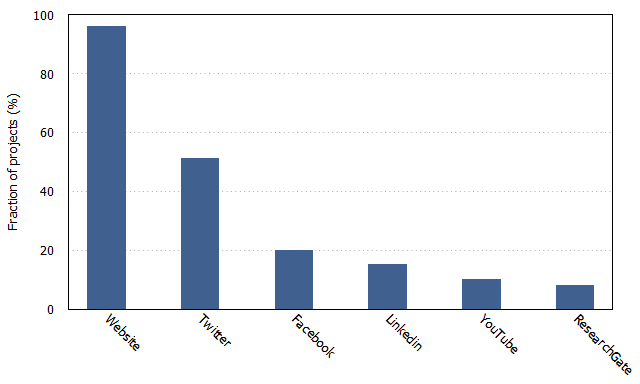
\includegraphics[scale=0.4]{Images/Social_media.png}
 \caption{Duration and allocated budget of Europe's Research and Innovation programmes (also known as Framework Programmes, FP). Budgets are expressed in billion Euros.}
 \label{Social_media}
 \end{center}
\end{figure}

